\documentclass[a4paper]{article}

\usepackage{fullpage} % Package to use full page
\usepackage{parskip} % Package to tweak paragraph skipping
\usepackage{tikz} % Package for drawing
\usepackage{amsmath}
\usepackage{hyperref}
\usepackage{graphicx}

\title{Iterated Prisoner's Dilemma}
\author{Ryan Day, Landon Willey, Landon Wright}
\date{October 9, 2018}

\begin{document}

\maketitle

\section{Introduction}
The prisoner's dilemma, originally created in 1950, has played an important role in the popularization of game theory. One of the most significant developments was Robert Axlerod's tournament with the iterated prisoner's dilemma game \cite{axelrod1981evolution}. In this paper, we recreate a similar situation with a few important differences. In our tournament, the payoff matrix has been set such that $2R=T+S$. We also play only a fixed set of nine simple strategies rather than a large set of user-submitted strategies. Finally, the results are based on six types of simulations: three with fixed numbers of trials (5, 100, and 200) and three with fixed probabilities that the game will continue on any given trial (0.75, 0.9, and 0.99).

\section{Methods}
% One page describing and justifying your strategy.
In addition to the strategies specified by the lab, we included a strategy of our own in the game. Our chosen strategy was ``two-tits-for-tat,'' which is a variation on tit-for-tat that plays cooperate on the first turn, tit-for-tat on the second, and then defects unless the opponent's last two moves were to cooperate.

While very simple, our strategy was carefully considered. As a starting point, we considered which strategies were successful in Axelrod's tournament. Our strategy met the majority of the criterion Axelrod proposed.

Our strategy is a ``nice'' strategy --- we don't defect until the opponent defects. This homogenizes the payoffs against all other nice strategies, since no player ever defects. We also play a strategy that quickly retaliates---as soon as an opponent defects, we defect on the next turn. Although the strategy is forgiving, it's not as forgiving as the normal tit-for-tat strategy, since we require the opponent to cooperate twice in a row before returning to a cooperative strategy. Tit-for-tat will never score higher than its opponent, while if the opponent defects, our strategy requires a repayment of twice the amount lost by being suckered before returning to mutual cooperation. This is a somewhat envious quality of our strategy, since after a defection, we never return to mutual cooperation without being allowed two temptation payoffs, resulting in a higher final payoff for our strategy.

We considered various other strategies before settling on this one. We thought about using a strategy that uses the first few moves to probe the opponent, but realized that this would severely reduce the payoff against any trigger strategies we played. Furthermore, we knew from Axelrod's results that some of the most successful strategies were generally simple strategies.  We wanted to create a strategy that would perform well against a variety of different strategies, not just the ones presented in this lab.  This was a major factor in the selection of our strategy as it will never trip a trigger strategy.  While this means that it doesn't benefit from the gains that can be achieved by taking advantage of strategies like always cooperate, it will also never receive the punishments that are associated with tripping a trigger strategy such as never forgive.

For the actual simulation of the tournament, we played a game with each player strategy against every other player strategy for each of the 6 game types: 5 games, 100 games, 200 games, P=0.75, P=0.9, and P=0.99. We repeated games with P values 30 times each in order to get more representative data. We could have also done multiple simulations for the games with a fixed number of iterations, but realizing that it would only have potential impacts on the results of games against the random strategy, we chose not to.

\section{Results and Analysis}
The game presented in this lab differed from the tournament proposed by Axelrod in that $2R = T + S$. Because of this discrepancy, as well as the inclusion of early-termination games, our strategy did not perform as well as we had hoped. The mean payoff for each strategy over all simulations is given in Table \ref{tab:allgameresults}. This data is stratified for different simulation types in Tables \ref{tab:trialresults} and \ref{tab:probresults}.  As can be seen in Table \ref{tab:allgameresults}, the overall best strategy was always defect followed by random, never forgive, and two-tits-for-tat (our strategy).  In Table \ref{tab:connectingLetters} we show the statistically significant differences between the different strategies, where any strategies that share the same letter are not statistically different at a p-value of 0.05 using an all pairs Tukey HSD test. Table \ref{tab:connectingLetters} reinforces our result that always defect is the clear winner, as it has the highest average score per round and is the only strategy that is statistically different than all other strategies.

\begin{table}[h!]
    \centering
    \begin{tabular}{lrr}
    Strategy            & Mean score per round & Variance score per round \\ \hline
    Always cooperate    & 2.68                 & 0.02                     \\
    Always defect       & 3.29                 & 0.58                     \\
    Never forgive       & 2.85                 & 0.07                     \\
    Pavlov              & 2.78                 & 0.03                     \\
    Random              & 2.90                 & 0.38                     \\
    Tit-for-tat         & 2.82                 & 0.03                     \\
    Tit-for-two-tats    & 2.76                 & 0.04                     \\
    Two-tits-for-tat    & 2.84                 & 0.05                     \\
    Win-stay-lose-shift & 2.75                 & 0.05                    
    \end{tabular}
    \caption{Means and variances of the score per round for each strategy against all opponents.}
    \label{tab:allgameresults}
\end{table}

The combined results for all games are also summarized in Figure \ref{fig:allgames} which shows the average per round payoff achieved by player 1, or the player on the bottom axis of the figure. As explained earlier, the majority of strategies are nice strategies; the result of this is that the large majority of games result in the player averaging the reward payoff of 3. 

\begin{table}[h]
    \centering
\begin{tabular}{lrrrrrr}
                    & \multicolumn{2}{c}{5 Games}   & \multicolumn{2}{c}{100 Games}  & \multicolumn{2}{c}{200 Games} \\
Strategy            & Mean & Variance & Mean & Variance & Mean & Variance \\ \hline
Always Cooperate    & 2.64        & 0.54    & 2.67   & 0.49      & 2.67   & 0.49    \\
Always defect       & 3.13        & 0.85    & 2.87   & 1.19      & 2.85   & 1.18    \\
Never forgive       & 2.82        & 0.16    & 2.93   & 0.14      & 2.95   & 0.17    \\
Pavlov strategy     & 2.96        & 0.50    & 2.81   & 0.25      & 2.81   & 0.25    \\
Random              & 3.04        & 0.46    & 2.65   & 0.59      & 2.64   & 0.67    \\
Tit for a tat       & 2.84        & 0.16    & 2.86   & 0.11      & 2.87   & 0.11    \\
Tit for two tats    & 2.76        & 0.26    & 2.81   & 0.15      & 2.82   & 0.14    \\
Two tits for a tat  & 2.89        & 0.17    & 2.91   & 0.12      & 2.92   & 0.13    \\
Win stay lose shift & 2.80        & 0.28    & 2.83   & 0.25      & 2.80   & 0.25                        
\end{tabular}
    \caption{Means and variances of the score per round for each strategy against all opponents for the games of known length.}
    \label{tab:trialresults}
\end{table}

This figure does give us some insights as to why the always defect strategy was so successful.  First we can note that against the always cooperate strategy it had a very high average utility, as we would expect. It also scored quite well against the Pavlov and win-stay-lose-shift strategies as they spent the majority of the time alternating between cooperate and defect, we would expect then the average utility of always defect against these strategies to be slightly higher than $T+P / 2 = 3.5$. In reality, the average utility per round of always defect against Pavlov and win-stay-lose-shift is 3.76 and 3.81 respectively.  These values are slightly higher than 3.5 due to low repeat number games as well as odd number games where the always defect player receives two temptation payouts.

\begin{table}[h]
    \centering
\begin{tabular}{lrrrrrr}
                    & \multicolumn{2}{c}{P=0.75} & \multicolumn{2}{c}{P=0.9} & \multicolumn{2}{c}{P=0.99} \\
Strategy            & Mean       & Variance      & Mean      & Variance      & Mean       & Variance      \\ \hline
Always Cooperate    & 2.65       & 0.53          & 2.67      & 0.47          & 2.67       & 0.45          \\
Always defect       & 3.64       & 1.21          & 3.30      & 1.12          & 2.95       & 1.07          \\
Never forgive       & 2.80       & 0.30          & 2.87      & 0.20          & 2.93       & 0.15          \\
Pavlov strategy    & 2.76       & 0.34          & 2.76      & 0.33          & 2.80       & 0.23          \\
Random              & 3.15       & 1.02          & 2.92      & 0.86          & 2.67       & 0.60          \\
Tit for a tat       & 2.79       & 0.26          & 2.81      & 0.19          & 2.85       & 0.12          \\
Tit for two tats    & 2.73       & 0.36          & 2.76      & 0.26          & 2.80       & 0.16          \\
Two tits for a tat  & 2.82       & 0.23          & 2.85      & 0.18          & 2.88       & 0.14          \\
Win stay lose shift & 2.73       & 0.40          & 2.78      & 0.28          & 2.79       & 0.24         
\end{tabular}
    \caption{Means and variances of the score per round for each strategy against all opponents for the games with a probability of continuing.}
    \label{tab:probresults}
\end{table}

Against the methods our strategy played against, the results were unremarkable in most cases. The results against nice strategies (always cooperate, tit-for-tat, tit-for-two-tats, Pavlov, win-stay/lose-shift, and never forgive) were all the same. Against one of the mean strategies, always defect, our strategy does no worse than tit-for-tat, which is the maximum possible for a nice strategy against always defect. Against the other potentially mean strategy, random, our strategy does slightly better than tit-for-tat, though not at the 0.5 significance level (see Table \ref{tab:connectingLetters}).





\begin{table}[]
    \centering
\begin{tabular}{llllll}
\textbf{Level}      &   &   &   &   & \textbf{Mean} \\ \hline
Always defect       & A &   &   &   & 3.29          \\
Random              &   & B &   &   & 2.9034468     \\
Never forgive       &   & B & C &   & 2.8459854     \\
Two-tits-for-tat    &   & B & C &   & 2.842517      \\
Tit-for-tat         &   & B & C &   & 2.8185575     \\
Pavlov              &   &   & C & D & 2.7811624     \\
Tit-for-two-tats    &   &   & C & D & 2.7604245     \\
Win-stay-lose-shift &   &   & C & D & 2.7530074     \\
Always cooperate    &   &   &   & D & 2.6821182    
\end{tabular}
    \caption{Connecting letters report, levels not connected by the same letter have a statistically significant difference at a two-sided p-value of 0.05 using an all pairs Tukey HSD test.}
    \label{tab:connectingLetters}
\end{table}

\begin{figure}
    \centering
    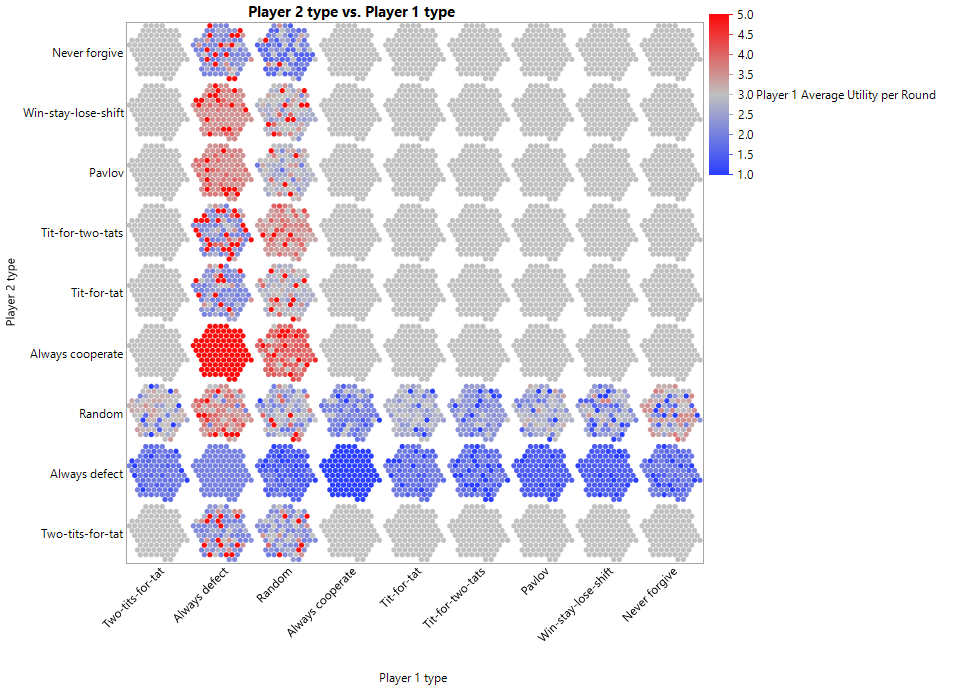
\includegraphics[width=\textwidth]{images/allGames.png}
    \caption{The results of every simulation run. Each cluster of points represents a match-up between two players.  Each point represents the results of one repeated play game colored by the average score of player 1}
    \label{fig:allgames}
\end{figure}

It is, however, of interest to examine the results of the our strategy versus the two mean strategies, which can be seen in Figure \ref{fig:usvsmean}.  As seen in the figure, our strategy typically scores around 3.25 per round in a game against a random strategy and typically scores around 2 per round in a game against an always defect strategy.  It is interesting that there are several outliers to the averages described.  These are the result of games that played very few rounds, and therefore the average per round value is heavily skewed.  This shows the importance of knowing what the likelihood of repeated play is, as when there is a low probability of repeated play, the always defect strategy is likely to win on a per round basis as there is comparatively little time for balance to be achieved.

\begin{figure}
    \centering
    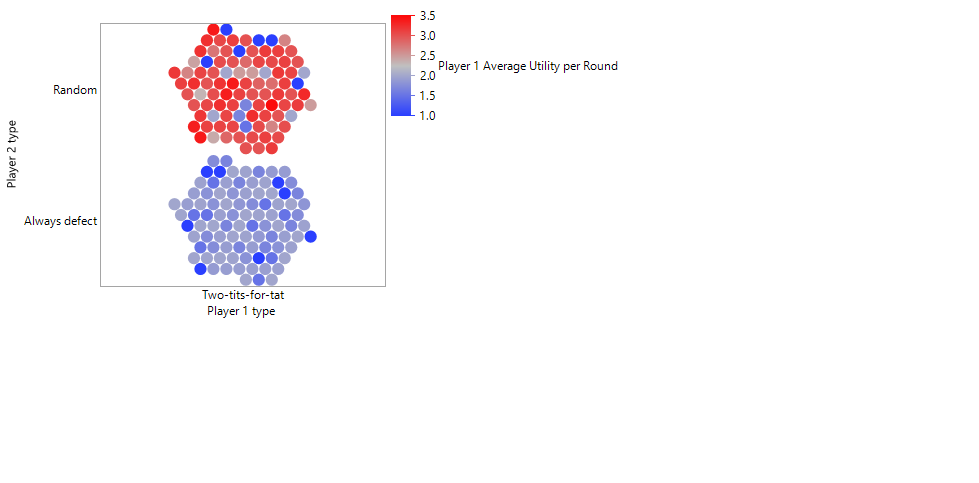
\includegraphics[clip, trim=0 4.3cm 9cm 0 ,width=0.75\textwidth]{images/usVsADRand.png}
    \caption{Results of two-tits-for-tat versus mean strategies}
    \label{fig:usvsmean}
\end{figure}

\begin{figure}
    \centering
    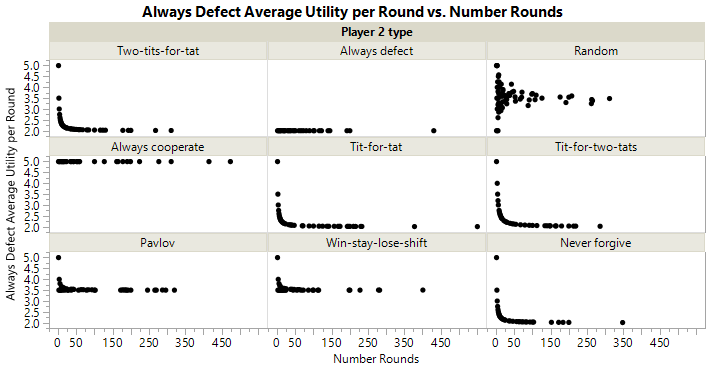
\includegraphics[width=\textwidth]{images/ADvsNRounds.png}
    \caption{Average payoff per round of always defect vs all other agents.  Note, that for nice agents the average payoff starts high, but within about 50 rounds settles to roughly 2. For random, Pavlov, and win-stay-lose-shift strategies the average payoff per round settles to around 3.5, larger than the reward payoff of 3.}
    \label{fig:advsrounds}
\end{figure}
This is very clearly illustrated in Figure \ref{fig:advsrounds} which shows how always defect strategy has a higher average score the fewer rounds that are played. This is because many strategies cooperate first, and the always defect strategy takes advantage of this. With more games played this effect is minimized, as strategies respond to always defect.


% Pavlov--defects when previous moves don't agree
% WSLS--switches on DC or DD.

% A description of the results for each number of trials listed above (5, 100, and 200); since this is a data intensive lab, take some time to present the information in an intelligible format.

% A description of the results for each of the probabilities above (0.75, 0.9, and 0.99); since this is a data intensive lab, take some time to present the information in an intelligible format.

\section{Conclusions}
The fact that always defect was a clear winner was a somewhat surprising result, since that strategy did not perform particularly well in Axelrod's tournament. Close analysis of the results reveals why this is. First, always defect happens to be the best response strategy against the majority of the other strategies (namely always cooperate, always defect, random, Pavlov, and win-stay-lose-shift). Because these make up more than half of the strategies in our tournament, it is no wonder that its payoff was higher than that of all other strategies.

Always defect also took advantage of the bias of the tournament toward shorter games. Of the six simulations run, most games were likely to be shorter, thus giving the first turn more weight in the final mean score per round.

After analyzing the game further, we realized that there was no benefit to the reward payoff compared to an endless cycle of temptation and sucker payoffs. With that information, and because always defect is a best response to so many of the other strategies in the game, a fairly simple learning agent could be developed to exploit the flaws in the game and do better than always defect. Within four moves, it can be determined whether or not an opponent is a tit-for-tat style agent or not. For tit-for-tat and tit-for-two-tats, the agent could play an endless cycle of defection and cooperation. Against regular tit-for-tat, this would result in an average payoff greater than or equal to than continual cooperation if the agent begins with defection. Against a more forgiving tit-for-two-tats agent, this cycle would exploit the agent, receiving the temptation payoff every other round.

This type of learning agent would trigger the never forgive strategy during the initial exploration stage, however the exploitation of the other agents would make up for the slight decrease in payoff against never forgive, thus allowing it to perform better than the always defect strategy. This strategy would only work because of the low number of trigger strategies in this game.

The above discussion reveals a very important fact about iterated prisoner's dilemma games. The strategy itself is not always the most important indicator of success in the game, but rather the assumptions under which the agents are playing (such as the likelihood of a future encounter) as well as the pool of opponents. For example, if the games were always 500 round encounters with a majority of tit-for-tat style agents, always defect would not be the most successful strategy.

In conclusion, in order to perform well within an iterated prisoner's dilemma scenario, it's important to know how the game will be played as well as who the opponents are. Without this information, a strategy that might otherwise perform well, such as our two-tits-for-tat strategy, can be easily beaten by a strategy that is able to exploit the tournament, such as always defect in this case.

\bibliographystyle{ieeetr}
\bibliography{bibliography}
\end{document}